\documentclass[../Report.tex]{subfiles}
\usepackage[italian]{babel}
\graphicspath{ {../../Images/} }

\begin{document}
    \chapter{Studio di fattibilità}
    \section{Contesto di utilizzo}
    Questa sezione mira ad identificare gli utenti della piattaforma e i loro compiti, in particolare enfatizzando la relazione tra i loro obiettivi (user goal) e le mansioni svolte (task). Inoltre, vengono individuati vincoli ambientali e tecnici rilevanti per le successive fasi di design.
        
        \subsection{Utenti previsti}
        Ci aspettiamo che gli utenti destinatari, che andranno ad utilizzare il sito Gioco.it, sono bambini che vogliono giocare ai vari mini giochi contenuti in esso ma in modo controllato rispettando il concetto di "different twins". Quindi, in questo caso il responsabile (i genitori/tutori) è diverso dall'utente (bambino).\\
        Abbiamo individuato due segmenti target di riferimento, in sintesi:
        \begin{itemize}
            \item Bambini di età compresa fra i 3 e i 18 anni che abbiano un minimo di dimestichezza con il dispositivo e con la navigazione internet. Interessati a giocare ai vari mini giochi presenti sul sito.
            \item Uomini/donne di età compresa fra i 30 e i 50 anni, il cui reddito è medio-basso (tutti ormai abbiamo almeno un dispositivo con navigazione internet) e che abbiano una buona dimestichezza con il dispositivo e con la navigazione internet. Interessati a far giocare il bambino a giochi prevalentemente educativi e bloccando quelli che ritengono inopportuni per l'età del bambino.
        \end{itemize} 

        \subsection{Compiti previsti}
        Durante le interviste sono emerse una serie di “idee per compiti” ricorrenti. Elaboriamo queste idee per produrre un elenco dei compiti più plausibili che il nostro sistema supporterà:
        \begin{itemize}
            \item Creazione di un profilo
            \item Login e logout dal sistema (anche con google o facebook)
            \item Visualizzare i giochi in tendenza
            \item Visualizzare i giochi in base a varie categorie e sottocategorie
            \item Giocare ai vari mini giochi
            \item Utilizzo di un parental control
            \item Commentare i giochi
            \item Aggiungere i giochi ai preferiti
            \item Aggiungere amici
            \item ecc...
        \end{itemize}

        \subsection{Vincoli ambientali e tecnici}
        \begin{itemize}
            \item \textbf{Vincoli tecnici:} trattandosi di una piattaforma web, è necessario che l'utente disponga di una connessione internet. Quindi supponiamo che tutti i nostri utenti possiedano almeno un personal computer (desktop o laptop) o smartphone con una connessione ad internet.
            \item \textbf{Vincoli culturali:} il sito è solo in lingua italiana e non si può accedere da un altro paese.
            \item \textbf{Vincoli ambientali:} la piattaforma è pensata per essere utilizzata nel tempo libero, pertanto l'ambiente di utilizzo più comune sarà la propria abitazione o un ambiente altrettanto confortevole e accogliente, senza alcun vincolo di tempo.
        \end{itemize}
        Ci aspettiamo quindi, che la maggior parte degli utenti utilizzi il sistema a proprio piacimento, in modo rilassato, esplorativo e possibilmente senza obiettivi.

    \section{Personas}
    Partendo dai nostri target segments, presentiamo quattro personas plausibili, due per ciascun target segments.\\
    \begin{table}[H]
        \begin{tabular}{|c|l|p{7cm}|}
            \hline
            \multirow{5}{*}{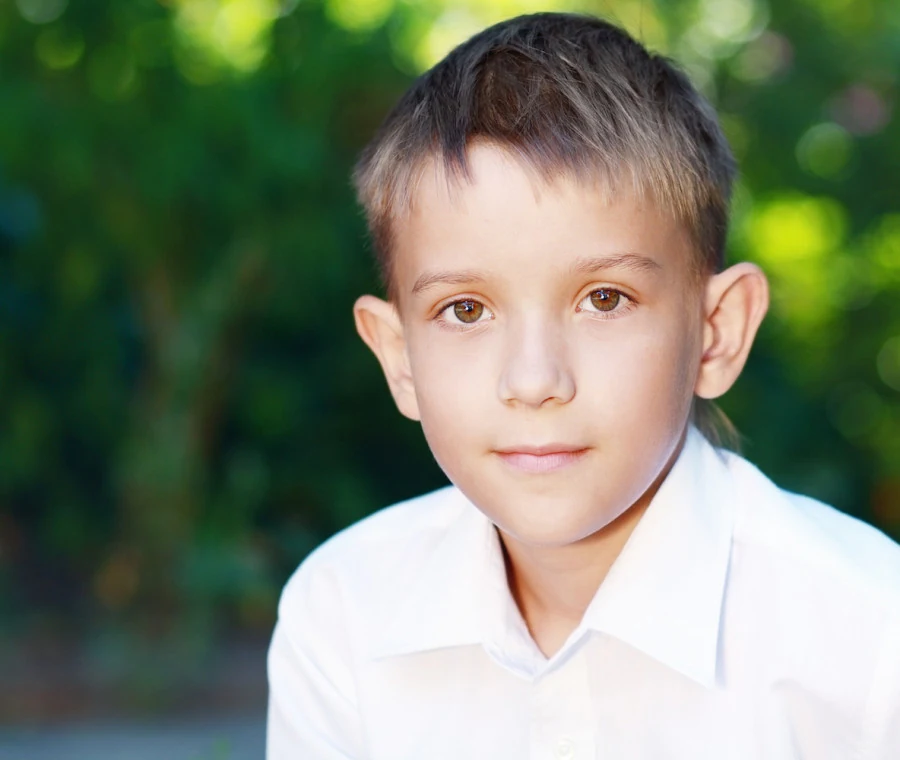
\includegraphics[width=5cm, height=5cm]{Mirko.jpg}} 
                & \textbf{Nome:} & Mirko Rossi\\ \cmidrule{2-3}
            & \textbf{Età:} & 10 \\ \cmidrule{2-3}
            & \textbf{Stato civile:} & Nubile \\ \cmidrule{2-3}
            & \textbf{Occupazione:} & \makecell{Studente \\ Mantenimento da parte dei genitori} \\ \cmidrule{2-3}
            & \textbf{Abilità tecinche:} & Usa il laptop del padre per fare ricerche scolastiche o per giocare. Gioca spesso con gli amici ed è imbattibile nei giochi d'azione, principalmente gli sparatutto. \\
            \hline
        \end{tabular}
    \end{table}

    \subsubsection{Descrizione}
    Mirko è un ragazzino di 10 anni che frequenta la quinta elementare nella scuola del suo paese. Ha una sorella di 15 anni ed è appassionata di moda. La madre, Susanna, lavora come maestra nella scuola elementare del loro piccolo borgo cittadino. Il padre, Antonio, esercita la professione di elettricista e spesso è fuori casa. Dopo aver fatto i compiti, Mirko, utilizza il laptop della madre per giocare a diversi videogiochi. La madre, essendo molto apprensiva nei confronti del figlio, tiene molto alla sua educazione, pertanto vorrebbe una maggiore sicurezza sugli usi del suo laptot.

    \vspace{1.5cm}

    \begin{table}[H]
        \begin{tabular}{|c|l|p{7cm}|}
            \hline
            \multirow{5}{*}{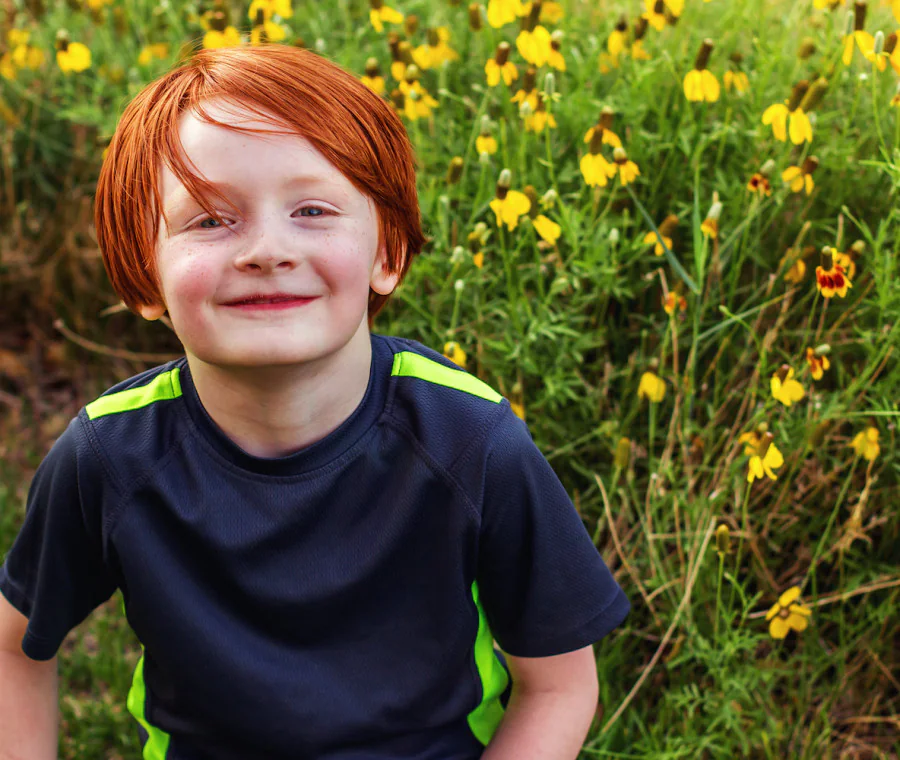
\includegraphics[width=5cm, height=5cm]{Gaetano.jpg}} 
                & \textbf{Nome:} & Gaetano Esposito\\ \cmidrule{2-3}
            & \textbf{Età:} & 6 \\ \cmidrule{2-3}
            & \textbf{Stato civile:} & Nubile \\ \cmidrule{2-3}
            & \textbf{Occupazione:} & \makecell{Studente \\ Mantenimento da parte dei genitori} \\ \cmidrule{2-3}
            & \textbf{Abilità tecinche:} &  È molto abile nel riconoscere i dinosauri ed ha imparato ad usare il computer grazie al padre.\\
            \hline
        \end{tabular}
    \end{table}

    \subsubsection{Descrizione}
    Gaetano è un bimbo di 6 anni, l'unico figlio di mamma Jennifer, parruchiera, e papà Claudio, Medico. È un bambino molto perspicace ed attento, ama la natura e gli animali e infatti per il suo quinto compleanno il padre gli ha regalato un bellissimo Golden Retriver di nome Pippo. La sua più grande passione sono i dinosauri, infatti riesce a riconoscerne molti grazie ai libri di storia.
    Gateano va due volte a settimana a seguire corsi di piscina, spinto dalla passione della madre, ex nuotatrice amatoriale.\\
    Il padre vorrebbe che imparasse giocando, ed è proprio per questo che gli permette di utilizzare il suo computer fisso per giocare a giochi educativi.

    \vspace{1.5cm}

    \begin{table}[H]
        \begin{tabular}{|c|l|p{7cm}|}
            \hline
            \multirow{5}{*}{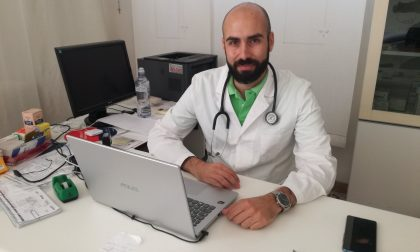
\includegraphics[width=5cm, height=5cm]{Claudio.jpg}} 
                & \textbf{Nome:} & Claudio Esposito\\ \cmidrule{2-3}
            & \textbf{Età:} & 45 \\ \cmidrule{2-3}
            & \textbf{Stato civile:} & Sposato \\ \cmidrule{2-3}
            & \textbf{Occupazione:} & \makecell{Medico di base \\ Mantenimento da parte dei genitori} \\ \cmidrule{2-3}
            & \textbf{Abilità tecinche:} &  Conosciuto in tutta la città per la sua professionalità e competenza. Ha un MacBook Pro che utilizza per lavorare e un computer fisso a casa per vedere film e seguire corsi di aggiornamento.\\
            \hline
        \end{tabular}
    \end{table}

    \subsubsection{Descrizione}
    Claudio è un uomo di 45 anni, sposato con una bellissima parrucchiera di nome Jennifer e hanno un bimbo di 6 anni, Gaetano, molto intelligente e appassionato di dinosauri e della natura. È uno dei più bravi medici di base della sua città e lo conoscono tutti con il soprannome di Ciruzzo, per le sue origini partenopee. Oltre al suo lavoro, gli piace cimentarsi nell'informatica e utilizza il suo computer fisso per seguire corsi di aggiornamento e guardare film e serie tv. Una delle sue serie tv preferite è l'anime Naruto, infatti lui e Gaetano passano ore davanti al pc a vedere le puntate.\\
    Claudio ci tiene molto all'educazione del figlio, ed è per questo che vorrebbe far giocare al figlio a dei giochi principalmente educativi, e date le passioni di Gaetano, giochi con animali sarebbero ottimi.

    \section{Scenari}
\end{document}